% ----------------------------------------------------------------------
% Presentación - Administración Actuarial (FES Acatlán, UNAM · 2026-1)
% Compilación: pdflatex (dos pasadas)
% ----------------------------------------------------------------------
\documentclass[aspectratio=169, 11pt]{beamer}

\usepackage[utf8]{inputenc}
\usepackage[T1]{fontenc}
\usepackage[spanish]{babel}
\usepackage{graphicx}
\usepackage{booktabs}
\usepackage{amsmath, amssymb}
\usepackage{tikz}
\usetikzlibrary{positioning, arrows.meta}

\definecolor{azulunam}{RGB}{0, 56, 101}
\definecolor{rojounam}{RGB}{201, 23, 30}
\definecolor{grisazul}{RGB}{240, 244, 248}

\newcommand{\bt}[1]{\textbf{#1}}

\usetheme{metropolis}
\metroset{block=fill, sectionpage=progressbar}

\setbeamercolor{palette primary}{bg=azulunam, fg=white}
\setbeamercolor{title}{fg=azulunam}
\setbeamercolor{frametitle}{bg=azulunam, fg=white}
\setbeamercolor{structure}{fg=azulunam}
\setbeamercolor{caption name}{fg=azulunam}

\title[Modelo de Otorgamiento de Crédito al 25\%]
      {Modelo de Otorgamiento de Crédito con Política de Aprobación al 25\%}
\subtitle{Scorecard de riesgo, comparación de modelos y clasificación de aprobados}
\author[Bárcena \& equipo]{Bárcena Romero Orlando · López Vélez Ricardo Alejandro\\
       García Mercado Karina · Carvajal Aguilar César Emir · Flores Frida}
\institute[FES Acatlán, UNAM]{Licenciatura en Actuaría · FES Acatlán, UNAM\\
       Administración Actuarial · Semestre 2026-1}
\date{\today}

\begin{document}

\begin{frame}[plain]
  \titlepage
\end{frame}

\begin{frame}{Agenda}
  \tableofcontents
\end{frame}

% ---------------------------------------------------------------------
\section{Contexto y problema de negocio}

\begin{frame}{El problema}
  \begin{itemize}
    \item \bt{292,849 solicitudes de crédito personal} (2007--2015).
    \item La institución \bt{sólo puede originar el 25\% del monto total
          solicitado} (presupuesto fijo).
    \item Pregunta de negocio: \bt{¿a cuáles solicitudes otorgar el crédito?}
    \item Después de originar, los aprobados se clasifican en
          \bt{Buenos} (pagaron) y \bt{Malos} (incumplieron).
  \end{itemize}

  \begin{alertblock}{Objetivo}
    Maximizar la calidad de la cartera aprobada (menos Malos) con el mismo
    presupuesto, usando un modelo de riesgo de crédito.
  \end{alertblock}
\end{frame}

\begin{frame}{Definición del fenómeno: ¿qué es un crédito Malo?}
  La base no trae el estatus final; se construye un \bt{proxy de cargo a
  pérdida} (\emph{charge-off}):

  \begin{itemize}
    \item \bt{Resuelto}: saldo principal $= 0$ (\texttt{out\_prncp}$=0$)
    \item \bt{Malo}: resuelto con recuperación o cobranza $>0$
          (\texttt{recoveries} / \texttt{collection\_recovery\_fee})
    \item \bt{Censurado}: saldo $>0$ (activo) $\Rightarrow$ se excluye
  \end{itemize}

  \begin{table}
    \small
    \caption*{Validez del proxy: mora por calificación interna}
    \begin{tabular}{lccccccc}
      \toprule
      Grade & A & B & C & D & E & F & G \\
      \midrule
      Mora (\%) & 3.3 & 6.7 & 9.7 & 14.0 & 18.3 & 23.9 & 22.9 \\
      \bottomrule
    \end{tabular}
  \end{table}
\end{frame}

\begin{frame}{Muestra}
  \begin{columns}
    \begin{column}{0.55\textwidth}
      \begin{itemize}
        \item \bt{Desarrollo}: resueltos emitidos antes de 2013-06
              ($n = 38{,}722$; mora 12.1\%)
        \item \bt{Out-of-time}: resueltos 2013-06 a 2015-01
              ($n = 37{,}450$; mora 9.0\%)
        \item Validación \emph{out-of-time} $\Rightarrow$ escenario real de
              uso (vintages nunca vistos)
      \end{itemize}
    \end{column}
    \begin{column}{0.45\textwidth}
      \begin{exampleblock}{Datos}
        \begin{itemize}
          \item 292,849 solicitudes, 42 variables
          \item 84,739 resueltos (28.9\%)
          \item 8,166 malos (tasa 9.6\%)
          \item 208,110 activos (censurados)
        \end{itemize}
      \end{exampleblock}
    \end{column}
  \end{columns}
  \vspace{0.5em}
  \tiny Solo información disponible al originar (sin \emph{look-ahead}).
\end{frame}

% ---------------------------------------------------------------------
\section{Metodología}

\begin{frame}{Flujo del proyecto}
  \begin{tikzpicture}[
      node distance=0.35cm and 0.5cm,
      box/.style={draw=azulunam, thick, rounded corners=2pt,
                  fill=grisazul, text width=2.6cm, align=center,
                  font=\footnotesize},
      arr/.style={-{Stealth[length=2.5mm]}, thick, color=azulunam}]
    \node[box] (d) {Datos y proxy\\ Bueno/Malo};
    \node[box, right=of d] (f) {Features de\\ originación};
    \node[box, right=of f] (m) {Comparativa:\\ Logit · RF · XGB};
    \node[box, right=of m] (s) {Scorecard\\ WoE + PDO};
    \node[box, below=of s] (a) {Aprobación 25\%\\ y clasificación};
    \node[box, below=of m] (e) {Métricas de\\ negocio};
    \draw[arr] (d) -- (f);
    \draw[arr] (f) -- (m);
    \draw[arr] (m) -- (s);
    \draw[arr] (s) -- (a);
    \draw[arr] (m) -- (e);
    \draw[arr] (a) -- (e);
  \end{tikzpicture}
\end{frame}

\begin{frame}{Métricas de negocio (riesgo de crédito)}
  \begin{columns}[T]
    \begin{column}{0.5\textwidth}
      \bt{Discriminación}
      \begin{itemize}
        \item \bt{KS}: separación máxima buenos vs malos
        \item \bt{AUROC}: $P(\text{score}_{\text{bueno}} >
              \text{score}_{\text{malo}})$
        \item \bt{Gini} $= 2\cdot$AUROC $- 1$
        \item \bt{CAP / Razón de Precisión}: concentración de malos
        \item \bt{Lift} por decil
      \end{itemize}
    \end{column}
    \begin{column}{0.5\textwidth}
      \bt{Calibración}
      \begin{itemize}
        \item \bt{LogLoss}
        \item \bt{Brier}
      \end{itemize}
      \vspace{1em}
      \bt{Decisión}
      \begin{itemize}
        \item Tasa de mora entre aprobados
        \item Buenos vs Malos aprobados
        \item Monto en riesgo evitado
      \end{itemize}
    \end{column}
  \end{columns}
\end{frame}

\begin{frame}{Scorecard de puntos}
  \begin{block}{Metodología estándar de la industria}
    \begin{itemize}
      \item Coarse classing por tramos
      \item $\mathrm{WoE}_i = \ln\!\big(\tfrac{\%Malos_i}{\%Buenos_i}\big)$ y
            Information Value para seleccionar variables
      \item Regresión logística sobre la matriz de WoE
      \item Puntos: $s = \text{offset} - \tfrac{\text{PDO}}{\ln 2}
            \ln(\text{odds})$, con PDO $=20$ (cada $+20$ pts duplica las
            odds de ser Bueno)
    \end{itemize}
  \end{block}
  \bt{Variables seleccionadas (IV y sin colinealidad):}
  {\small \texttt{grade} · \texttt{term\_months} · \texttt{income\_per\_loan}
  · \texttt{revol\_util}}
\end{frame}

% ---------------------------------------------------------------------
\section{Resultados}

\begin{frame}{Comparativa de modelos (out-of-time)}
  \begin{table}
    \small
    \begin{tabular}{lcccccc}
      \toprule
      Modelo & KS & AUROC & Gini & AR & LogLoss & Brier \\
      \midrule
      Regresión Logística & 0.294 & \bt{0.698} & \bt{0.396} & \bt{0.396}
             & 0.703 & 0.251 \\
      Random Forest        & 0.294 & 0.697 & 0.393 & 0.393 & 0.639 & 0.224 \\
      XGBoost              & 0.282 & 0.690 & 0.380 & 0.380 & \bt{0.298} & \bt{0.084} \\
      \bottomrule
    \end{tabular}
  \end{table}
  \begin{itemize}
    \item Los tres modelos discriminan de forma comparable.
    \item \bt{XGBoost} destaca en calibración; \bt{logística} es la más
          estable y la base del scorecard.
  \end{itemize}
\end{frame}

\begin{frame}{Scorecard: desempeño y deciles}
  \begin{columns}
    \begin{column}{0.5\textwidth}
      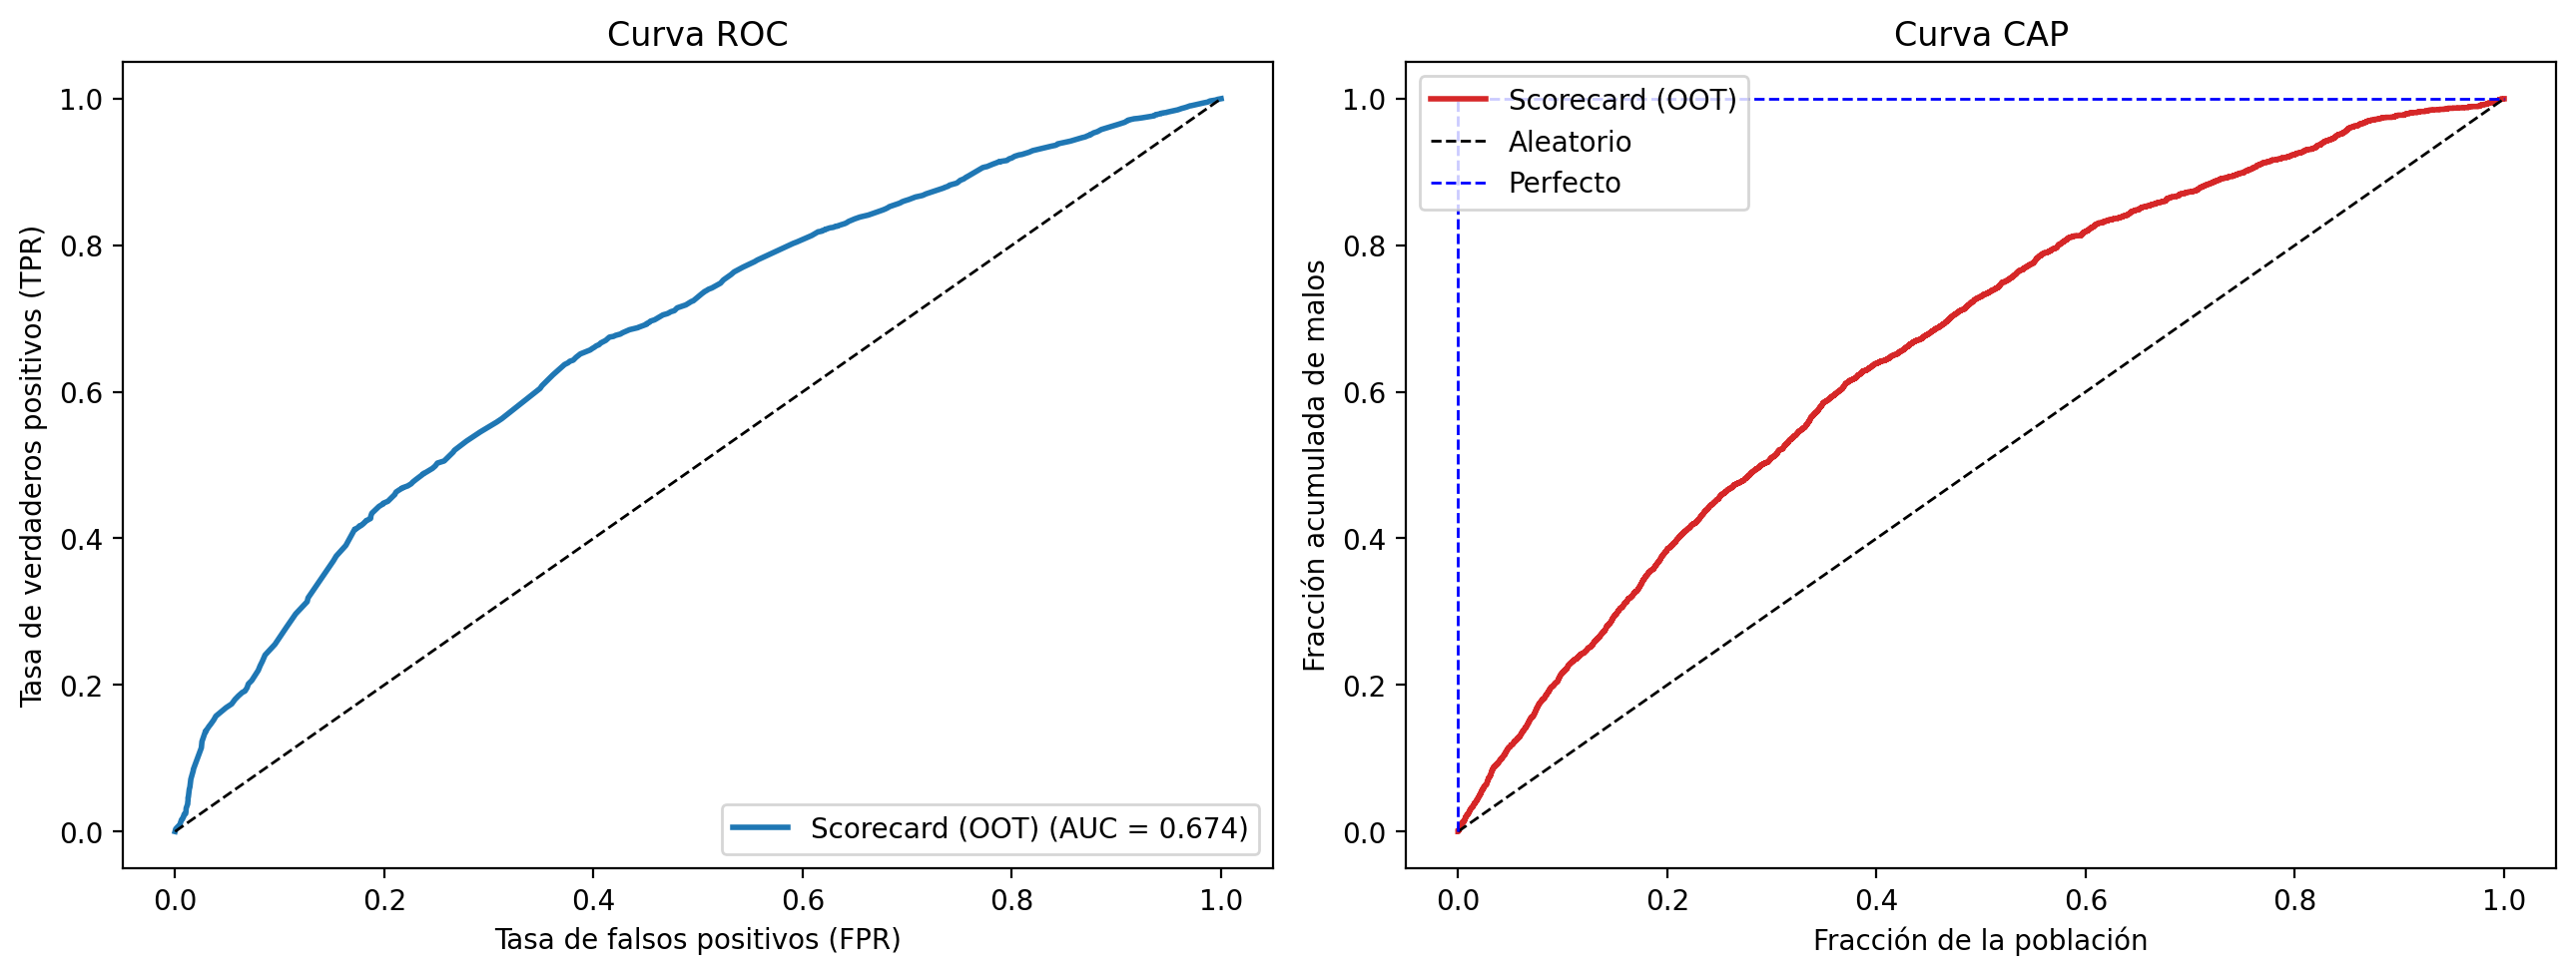
\includegraphics[width=\linewidth]{figures/scorecard_roc_cap.png}
      \tiny ROC y CAP del scorecard (OOT): AUROC 0.674, Gini 0.349, KS 0.265
    \end{column}
    \begin{column}{0.5\textwidth}
      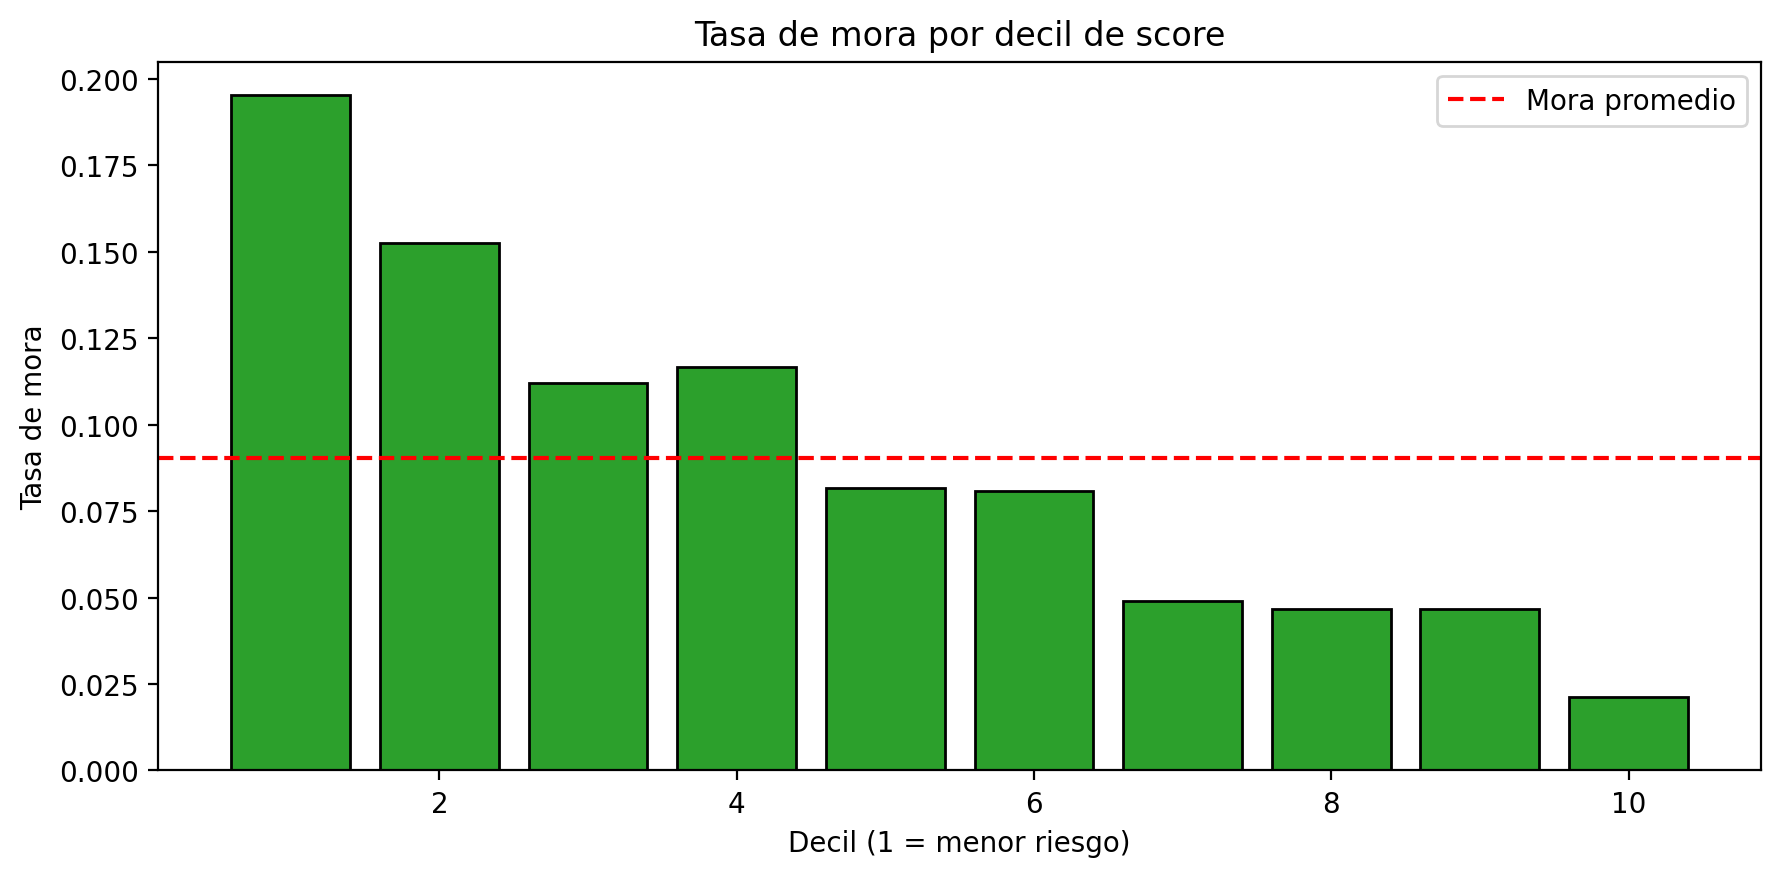
\includegraphics[width=\linewidth]{figures/deciles_mora.png}
      \tiny Mora por decil: 2.1\% (mejor) a 19.6\% (peor)
    \end{column}
  \end{columns}
\end{frame}

\begin{frame}{Resultado de la política de aprobación al 25\%}
  Presupuesto \bt{US\$ 133.7M} = 25\% de los US\$ 534.7M solicitados (OOT).

  \begin{table}
    \small
    \begin{tabular}{lrrrrr}
      \toprule
      Política & Aprobados & Monto (US\$) & Buenos & Malos & Morosidad \\
      \midrule
      \bt{Scorecard} & 9,447 & 133.7M & 9,107 & \bt{340} & \bt{3.6\%} \\
      Aleatorio        & 9,402 & 133.7M & 8,574 & 828 & 8.8\% \\
      Aprobar todos    & 37,450 & 534.7M & 34,069 & 3,381 & 9.0\% \\
      \bottomrule
    \end{tabular}
  \end{table}

  \begin{alertblock}{Impacto de negocio}
    El mismo presupuesto genera \bt{2.5 veces menos créditos incobrables}
    con el scorecard (340 vs 828 vs 3,381).
  \end{alertblock}
\end{frame}

% ---------------------------------------------------------------------
\section{Conclusiones}

\begin{frame}{Conclusiones}
  \begin{itemize}
    \item El proxy de charge-off es un fenómeno válido y consistente con la
          calificación interna.
    \item Logística, RF y XGBoost rinden de forma comparable (AUROC 0.69--0.70);
          se elige el \bt{scorecard de 4 variables} por interpretabilidad y
          auditabilidad, conservando 97\% del poder del modelo completo.
    \item Con la restricción del 25\%, la selección por score \bt{reduce la
          mora aprobada de 9.0\% a 3.6\%} (2.5$\times$ menos incobrables).
  \end{itemize}

  \vspace{0.5em}
  \bt{Recomendaciones}: monitoreo mensual de KS/Gini, buró externo,
  corte de score mínimo, análisis de supervivencia y \emph{risk-based
  pricing}.
\end{frame}

\begin{frame}[plain]
  \centering
  \vspace{1.5cm}
  {\Large\bfseries\color{azulunam} ¡Gracias!}\\[0.8cm]
  {\large Administración Actuarial · Semestre 2026-1}\\[0.3cm]
  FES Acatlán, UNAM\\[1cm]
  Código, informe y reproducción: \texttt{src/}, \texttt{reports/},
  \texttt{notebooks/}
\end{frame}

\end{document}